
The production of $WZ$ in association with a heavy flavor jet represents an important background for many major analyses. This includes any process with multiple leptons and b-jets in the final state, such as $t\bar{t}H$, $t\bar{t}W$, and $t\bar{t}Z$. While precise measurements have been made of inclusive $WZ$ production \cite{WZ_36}, $WZ$ + heavy flavor remains poorly understood. This is largely because the QCD processes involved in the production of the b-jet make it difficult to simulate accurately. This introduces a large uncertainty for analyses that include this process as a background.  

\begin{figure}[H]
  \centering
  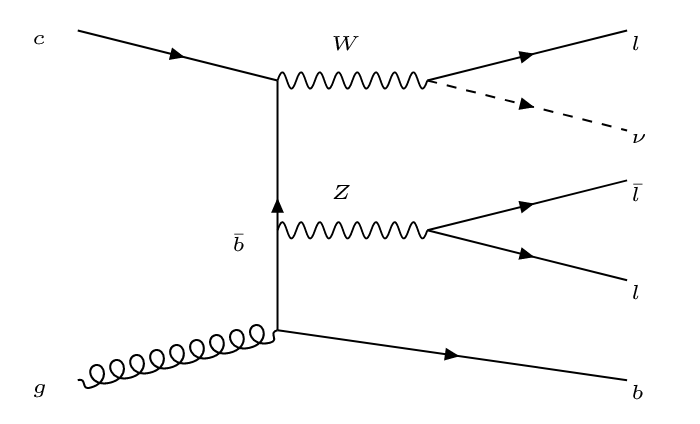
\includegraphics[width=0.55\linewidth]{figures/wz_3l.png}%                                                                 
  \includegraphics[width=0.39\linewidth]{figures/wz_bbar.JPG}
  \caption{Example Feynman diagrams of WZ + heavy flavor production}
  \label{fig:wz_feynman}
\end{figure}

We perform a study of the fully leptonic decay mode of this channel; that is, events where both the W and Z decay leptonically. Because WZ has no associated jets at leading order, while the major backgrounds for this channel tend to have high jet multiplicity, events with more than two jets are rejected. This gives a final state signature of three leptons and one or two jets.

Events that meet a preselection criteria are sorted into regions based on the b-tagging score of their associated jets. This is done to separate $WZ$ + b-jet events from $WZ$ + charm and $WZ$ + light jets. These regions are fit to data in order to make a more accurate estimate of the contribution of $WZ$ + heavy-flavor, where heavy-flavor jets include b-jets and charm jets. The full Run-2 dataset collected by the ATLAS detector, representing 139 $fb^{-1}$ of data from pp collisions at $\sqrt{s} = 13$ TeV, is used for this study.

The fiducial volume at particle level is defined based on the number of stable leptons and jets in each event. Three light leptons with total charge $\pm$1 and one or two associated jets are required. Only leptons which do not originate from hadron or $\tau$ decays are considered. The phase space definitions use dressed kinematics of the final state particles. Leptons are dressed by summing the momentum of photons within a cone of $\Delta R < 0.1$ of the lepton to correct the leptons energy. Particle level jets are reconstructed using the anti-$k_t$ algorithm with a radius of $R=0.4$. The kinematic selection applied to these objects is summarized below:

\begin{itemize}
\item Three light leptons with total charge $\pm$1, $|\eta| < 2.5$
\item OS lepton with \pt$>$10 GeV, SS leptons with \pt$>$20 GeV
\item One OSSF lepton pair with $|M(ll)-91.2\ GeV| < 10\ GeV$
\item One or two associated truth jets with $p_T >$25 GeV, $|\eta| < 2.5$, $R<0.4$
%\item At least one truth b-jet or one charm jet
\end{itemize}

The result of the fit is used to extract the cross-section in this fiducial region for WZ + $b$ and WZ + $c$ with one associated jet, and WZ + $b$ and WZ + $c$ with two associated jets, where the number and flavor of the jets is determined at particle level. Events with both charm and b-jets are counted as WZ + $b$. The analysis reports a cross-section measurement of WZ + $b$ and WZ + $c$, along with their correlations, for both 1-jet and 2-jet exclusive regions. Normalization factors, representing how the MC prediction differs from the observed result in the fit regions, are also reported.

Section \ref{sec:data} details the data and Monte Carlo (MC) samples used in the analysis. The reconstruction of various physics objects is described in Section \ref{sec:obj}. Section \ref{sec:evt_selection} describes the event selection applied to these samples, along with the definitions of the various regions used in the fit. The multivariate analysis techniques used to separate the tZ background from WZ + heavy flavor are described in Section \ref{sec:tZ_bdt}. Section \ref{sec:sys} describes the various sources of systematic uncertainties considered in the fit. Finally, the results of the analysis are summarized in Section \ref{sec:results}, followed by a brief conclusion in Section \ref{sec:conclusion}.


